 \documentclass[tikz,border=1mm]{standalone}

\usepackage{pgfplots}
\usetikzlibrary{patterns,decorations.pathmorphing,positioning}
\usetikzlibrary{calc,patterns,decorations.pathmorphing,decorations.markings}
\usetikzlibrary{external}
\pgfplotsset{compat=1.6}
\begin{document}
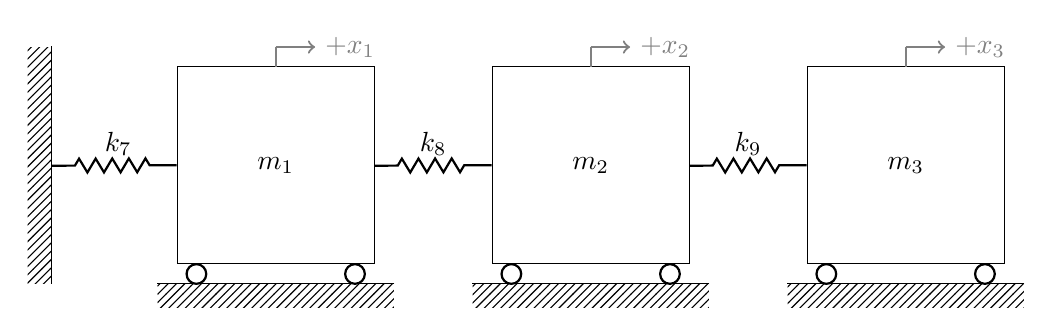
\begin{tikzpicture}
\tikzstyle{spring}=[thick,decorate,decoration={zigzag,pre length=0.3cm,post length=0.3cm,segment length=6}]
\tikzstyle{damper}=[thick,decoration={markings,  
  mark connection node=dmp,
  mark=at position 0.5 with 
  {
    \node (dmp) [thick,inner sep=0pt,transform shape,rotate=-90,minimum width=15pt,minimum height=3pt,draw=none] {};
    \draw [thick] ($(dmp.north east)+(2pt,0)$) -- (dmp.south east) -- (dmp.south west) -- ($(dmp.north west)+(2pt,0)$);
    \draw [thick] ($(dmp.north)+(0,-5pt)$) -- ($(dmp.north)+(0,5pt)$);
  }
}, decorate]
\tikzstyle{ground}=[fill,pattern=north east lines,draw=none,minimum width=0.75cm,minimum height=0.3cm]
% Mass 1
\begin{scope}[xshift=7cm]
\node (M) [minimum width=2.5cm, minimum height=2.5cm] {$m_{1}$};
\draw (-1.25,-1.25) rectangle (1.25,1.25);
\node (ground) [ground,anchor=north,yshift=-0.25cm,minimum width=3.cm] at (M.south) {};
\draw (ground.north east) -- (ground.north west);
\draw [thick] (M.south west) ++ (0.25cm,-0.125cm) circle (0.125cm)  (M.south east) ++ (-0.25cm,-0.125cm) circle (0.125cm);
\node (wall) [ground, rotate=-90, minimum width=3cm,yshift=-3cm] {};
\draw (wall.north east) -- (wall.north west);
% Spring + spring constant
\draw [spring] ($(wall.east)+(0.15,1.5cm)$) -- ($(M.west)+(0,0cm)$);
\node [above] at (-2,0) {$k_7$};
% Coordinate System
\draw [thick,gray,->] (0,1.5) -- (0.5,1.5) node[right] {$+x_{1}$};
\draw [thick,gray,-] (0,1.25) -- (0,1.5);
\end{scope}
% Mass 2
\begin{scope}[xshift=11cm]
\node (M) [minimum width=2.5cm, minimum height=2.5cm] {$m_{2}$};
\draw (-1.25,-1.25) rectangle (1.25,1.25);
\node (ground) [ground,anchor=north,yshift=-0.25cm,minimum width=3.cm] at (M.south) {};
\draw (ground.north east) -- (ground.north west);
\draw [thick] (M.south west) ++ (0.25cm,-0.125cm) circle (0.125cm)  (M.south east) ++ (-0.25cm,-0.125cm) circle (0.125cm);
% Spring + Spring Constant
\draw [spring] ($(wall.east)+(4.25,1.5cm)$) -- ($(M.west)+(0,0cm)$);
\node [above] at (-2,0) {$k_8$};
% Coordinate System
\draw [thick,gray,->] (0,1.5) -- (0.5,1.5) node[right] {$+x_{2}$};
\draw [thick,gray,-] (0,1.25) -- (0,1.5);
\end{scope}
% Mass 3
\begin{scope}[xshift=15cm]
\node (M) [minimum width=2.5cm, minimum height=2.5cm] {$m_{3}$};
\draw (-1.25,-1.25) rectangle (1.25,1.25);
\node (ground) [ground,anchor=north,yshift=-0.25cm,minimum width=3.cm] at (M.south) {};
\draw (ground.north east) -- (ground.north west);
\draw [thick] (M.south west) ++ (0.25cm,-0.125cm) circle (0.125cm)  (M.south east) ++ (-0.25cm,-0.125cm) circle (0.125cm);
% Spring + Spring Constant
\draw [spring] ($(wall.east)+(8.25,1.5cm)$) -- ($(M.west)+(0,0cm)$);
\node [above] at (-2,0) {$k_9$};
% Coordinate System
\draw [thick,gray,->] (0,1.5) -- (0.5,1.5) node[right] {$+x_{3}$};
\draw [thick,gray,-] (0,1.25) -- (0,1.5);
\end{scope}
\end{tikzpicture}
\end{document}
